\documentclass{article}
\usepackage{lipsum}
\usepackage{fancyhdr}
\usepackage{graphicx}
\usepackage[all]{xy}
\usepackage{amsmath, amsthm, latexsym, amssymb, graphicx,color,cite,mathabx,enumerate,mathrsfs}
\usepackage[left=2.0 cm,right=2.0cm,top=3cm,bottom=3cm]{geometry}
\pagenumbering{arabic}
\pagestyle{fancy}
\rhead{HUAN Q. BUI}
\usepackage{dsfont}
\newtheorem{theorem}{Theorem}
\newtheorem{fact}{Fact}
\newtheorem{lemma}{Lemma}
\newtheorem{definition}{Definition}
\newtheorem{corollary}{Corollary}
\newtheorem{proposition}{Proposition}
\newtheorem{remark}{Remark}
\newtheorem{notation}{Notation}
\newtheorem{example}{Example}
\newtheorem{non-example}{Non-example}
\renewcommand{\Re}{\operatorname{Re}}%%redefined Re and Im
\renewcommand{\Im}{\operatorname{Im}}
\newcommand{\tr}{\operatorname{tr}}
\renewcommand{\det}{\operatorname{det}}
\newcommand{\cadlag}{\textit{c\'{a}dlag} }
\newcommand{\E}{\mathbb{E}}%notation for expectation
\newcommand{\unit}[1]{\overline{\underline{#1}}}%notation for the unit contraction function

\usepackage{amsmath}
%\usepackage{svgcolor}
\usepackage[svgnames]{xcolor}
\usepackage[framemethod=tikz]{mdframed}


\newcommand{\p}{\partial}
\newcommand{\R}{\mathbb{R}}
\newcommand{\C}{\mathbb{C}}
\newcommand{\lag}{\mathcal{L}}
\newcommand{\I}{\mathcal{I}}
\newcommand{\K}{\mathcal{K}}
\newcommand{\F}{\mathcal{F}}
\newcommand{\w}{\omega}
\newcommand{\lam}{\lambda}
\newcommand{\al}{\alpha}
\newcommand{\be}{\beta}
\newcommand{\x}{\xi}

\newcommand{\W}{\mathcal{W}}

\newcommand{\f}[2]{\frac{#1}{#2}}

\newcommand{\ift}{\infty}

\newcommand{\lp}{\left(}
\newcommand{\rp}{\right)}

\newcommand{\lb}{\left[}
\newcommand{\rb}{\right]}

\newcommand{\lc}{\left\{}
\newcommand{\rc}{\right\}}

\usepackage{csquotes}
\usepackage{caption}



\title{{Calculus of Variations}\\{\&}\\{Partial Differential Equations}}
\author{Huan Q. Bui}
\date{May 18, 2019}
\begin{document}
\pagenumbering{roman}
\maketitle
\begin{figure}[h!]
\centering
\includegraphics[scale=0.53,angle=270]{intro.eps}
\captionsetup{labelformat=empty}
\caption{Spot the Cycloid!}
\end{figure}



\newpage
\tableofcontents
\newpage
\pagenumbering{arabic}





\section{Introduction}

\noindent From an applied viewpoint, calculus of variations poses a fascinating alternative approach to solving optimization problems: by considering small deviations from a solution (variations) and finding solutions based on what makes non-solutions sub-optimal. In a way, the idea of calculus of variations is much like the scientific process where the necessary conditions for a solution to a problem or a scientific theory of a natural phenomenon is often obtained by trial (deviations from the true solution) and error (how a deviation from the solution is penalized). It is thus not surprising that calculus of variation gives a \textit{natural} and appealing way for finding physical laws. Calculus of variations appears in almost all corners of physics, often under the name of the Principle of Least Action: from Lagrangian's formalism of classical mechanics to the foundations of classical and quantum field theory, the Standard Model of physics and its extension (SME). \\


In physics, calculus of variations and differential equations go almost hand-in-hand. Physical laws are often written as differential equations. For example, Newton's law of gravitation relates the spatial gradient of a force field to the rate of change of the velocity of a particle in the field. On the other hand, many theories such as the Schr\"{o}dinger's equation or the Eintein's field equations, while originally postulated, has been shown from time to time to be obtainable from variational methods. For instance, the Einstein's field equations can be obtained through variational methods applied to the metric tensor $g_{\mu\nu}$. \\


This paper attempts to provide an overview of the connection between calculus of variations and (partial) differential equations. Starting with some simple  physically-motivated examples, this paper will derive the Euler-Lagrange equations and show how physical laws, expressed as a differential equation, can be generally obtained from variational methods in Lagrangian mechanics and beyond. Through an initial boundary value problem with Laplace's equation and inhomogeneous boundary condition, the paper will also show how this problem in partial differential equation can be written as a minimization problem that is solvable by variational methods. A similar problem in electrostatics will be considered to further illustrate this idea. \\

The final section of this paper shows a glimpse into the much more profound mathematical connection between partial differential equation and calculus of variations. In particular, the paper will briefly discuss how some of the questions in calculus of variations and partial differential equations are answered in functional analysis.  


\section{Calculus of Variations}
\subsection{Euler-Lagrange Equation}

In this section, we will look at how calculus of variations is applied to a simple problem, and how the Euler-Lagrange equation arises as a necessary condition for a solution to an optimization problem. \\

Suppose we want to find the shortest arc joining two points on a plane. We are certain that the arc is a straight line. But how is a straight line joining two points is the shortest arc? The idea of calculus of variations is to consider a solution $\bar{y}(x)$ that minimizes the distance $S$ between the two points, say $A(x_1,y_1)$ and $B(x_2,y_2)$, and some deviation $\eta(x)$ from this correct curve $\bar{y}(x)$. Any deviation from the correct path associated with $\eta(x)$ can thus be written as
\begin{align}
y(x) = \bar{y}(x) + \epsilon \eta(x)
\end{align}
where $\epsilon$ is a constant parameter controlling for the magnitude of the deviation $\eta(x)$. Since we want the end points of any general path to be the same as the correct path, it is required that $\eta(x_1) = \eta(x_2) = 0$.\\

The distance $S(\epsilon)$ between $A$ and $B$ for any given $\eta(x)$ can be found by a little bit of calculus:
\begin{align}
S(\epsilon) = \int^{x_2}_{x_1}\sqrt{1 + \left(\frac{dy}{dx}\right)^2}\,dx.
\end{align}

Before solving this problem, let us think about a more general case. Let the integrand be $f = f(y',y,x) = f(\bar{y}'+\epsilon\eta',y+\epsilon\eta,x)$, where $x$ is the independent variable and $f$ is sufficiently differentiable. Since we require that $S(\epsilon)$ is minimized, $dS(\epsilon)/d\epsilon = 0$. Thus it is necessary that
\begin{align}\label{exp}
0 &= \f{dS}{d\epsilon} \nonumber\\ 
&= \f{d}{d\epsilon}\int^{x_2}_{x_1}f(\bar{y}'+\epsilon\eta',y+\epsilon\eta,x)\,dx \nonumber\\
&= \int^{x_2}_{x_1}\f{d}{d\epsilon}f(\bar{y}'+\epsilon\eta',y+\epsilon\eta,x)\,dx \nonumber\\
&= \int^{x_2}_{x_1}\eta'\f{\p f}{\p y'} + \eta\f{\p f}{\p y}\,dx 
\end{align}

Consider the first term in the integrand. Integrating by parts gives.
\begin{align}\label{bounds}
\int^{x_2}_{x_1}\eta'\f{\p f}{\p y'} \,dx
&= \eta\f{\p f}{\p y'}\bigg\vert_{x_1}^{x_2} -  \int^{x_2}_{x_1}  \f{d}{dx}\f{\p f}{\p y} \,dx \nonumber\\
&= -  \int^{x_2}_{x_1}  \f{d}{dx}\f{\p f}{\p y} \,dx,
\end{align} 
where the boundary term vanishes due to the constraint $\eta(x_1) = \eta(x_2) = 0$. From \eqref{exp} and \eqref{bounds}, we have
\begin{align}\label{euler}
0 = \int^{x_2}_{x_1} \eta\lp \f{\p f}{\p y} - \f{d}{dx}\f{\p f}{\p y'}  \rp\,dx. 
\end{align}

Now, because we require that $\bar{y}(x)$ minimizes $S$ and that this holds for any deviation $\eta(x)$ from $\bar{y}(x)$, the integrand in \eqref{euler} must be zero. Thus, we obtain the \textbf{Euler-Lagrange equation}:
\begin{align}
\boxed{\f{\p f}{\p y} - \f{d}{dx}\f{\p f}{\p y'} = 0}
\end{align}

Back to our original problem with finding the shortest arc joining two points on a plane. We have that
\begin{align}
f(y',y,x) = \sqrt{1 + \lp\f{dy}{dx}\rp^2}.
\end{align}
Thus,
\begin{align}
\begin{cases}
\f{\p f}{\p y} = 0\\
\f{\p f}{\p y'} = \f{1}{2}\f{2y'}{\sqrt{1 + y'^2}} = \f{y'}{\sqrt{1 + y'^2}}.
\end{cases}
\end{align}
By the Euler-Lagrange equation, 
\begin{align}
0 - \f{d}{dx}\lp \f{y'}{\sqrt{1 + y'^2}} \rp = 0,
\end{align}
i.e., $(y')\sqrt{1 + y'^2}$ is some constant $C$, i.e.,
\begin{align}
y' &= C\sqrt{1 + y'^2}\nonumber\\
y'^2 &= C^2(1+y'^2)\nonumber\\
(1 - C^2)y'^2 &= C^2.
\end{align} 
This says $y' = dy/dx$ is a constant, which means 
\begin{align}
y(x) = ax + b
\end{align} 
for some constants $a,b$. This is nothing but an equation for a line on a plane, as expected. Of course, this is a motivating example for that we can see how the Euler-Lagrange equation arises. The problem of minimizing the distance between two points on a plane certainly does not require calculus of variations, but we shall see in the following example how the Euler-Lagrange equation can come in handy.

\subsection{The Brachistochrone Problem}

Perhaps one of the most well-known examples of the superiority of Lagrangian mechanics over conventional methods in Newtonian mechanics is the problem of finding the frictionless path for an object to slide down with the shortest (\textit{brachistos}) amount of time (\textit{chronos}). This problem was originally posed by John Bernoulli in 1696 and attracted the attention of many eminent mathematicians and physicists at the end time including Isaac Newton, Leibniz, L'Hopital, and Johann Bernoulli, John Bernoulli's brother. \\

Here we are minimizing time, so we must first find an express for time. Assuming that the object travels from initial height $c$ to final height $d$. With a bit of calculus and basic mechanics, we have
\begin{align}\label{time}
T &= \int_{0}^{L} \frac{ds}{v} = \int_c^d \f{\sqrt{1 + x'^2}}{v}\,dy,
\end{align}
where $v$ is the speed of the object. To express the speed $v$ in terms of height $y$, we use conservation of energy. Assuming the total energy is zero and is conserved, we get
\begin{align}
[\text{Potential Energy}] + [\text{Kinetic energy}] = - mgy + \frac{1}{2}mv^2 = 0.
\end{align}
Note that the sign convention is so that potential energy is negative. Thus,
\begin{align}
v = \sqrt{2gy}.
\end{align}
Putting this into \eqref{time}, we get
\begin{align}
T = \frac{1}{\sqrt{2g}}\int^d_c \sqrt{\f{1 + x'^2}{y}}\,dy.
\end{align}
Let the integrand be $f[x',x,y]$, by the Euler-Lagrange equation we have
\begin{align}
\frac{\p f}{\p x} - \f{d}{dy}\f{\p f}{\p x'} = 0 - \frac{d}{dy}\f{1}{\sqrt{y}}\cdot \f{x'}{\sqrt{1 + x'^2}}  = 0.
\end{align}
Thus,
\begin{align}
\f{x'}{\sqrt{y(1+x'^2)}} = \f{1}{2a}
\end{align}
where $a$ is some non-zero constant. It follows that 
\begin{align}
0 &= (2ax')^2 - y(1+x'^2)\nonumber\\
&= x'^2(2a-y) - y.
\end{align}
Rearranging and integrating both sides, we get
\begin{align}
x = \int_c^d \sqrt{\frac{y}{2a-y}}\,dy.
\end{align}
Now, we notice that $0 \leq y \leq 2a$, so we can make the substitution $y = a(1-\cos\theta)$. Then, $dy = a\sin\theta\,d\theta$. And so,
\begin{align}
x 
&= \int \sqrt{\frac{1-\cos\theta}{1 + \cos\theta}}a\sin\theta\,d\theta \nonumber\\
&= a\int \sqrt{\frac{(1 - \cos\theta)^2}{1 - \cos^2\theta}}\sin\theta\,d\theta \nonumber\\
&= a\int \f{1-\cos\theta}{\sin\theta}\sin\theta\,d\theta\nonumber\\
&= a\int 1-\cos\theta \,d\theta\nonumber\\
&= a(\theta - \sin\theta) + C.
\end{align}
We can define locations such that initially, the object is at $(x,y) = (0,0)$. This gives $C = 0$. And so,
\begin{align}
\begin{cases}
x = a(\theta - \sin\theta)\\
y = a(1-\cos\theta).
\end{cases}
\end{align}
This is the parameterization for a \textbf{cycloid}, the curved traced by a point on a circle as is rolls without slipping in a straight line. \\

\begin{figure}[h!]
	\centering
	\includegraphics[scale=0.35, angle=180]{cycloid.eps}
\end{figure}

It is now clear that variation method can give us an elegant way to find a solution describing a physical system that is not very obvious to us from the start. One might find that attempting this problem using only Newtonian mechanics is much more challenging. 


\subsection{Remark: Necessary and (almost) sufficient conditions}
It is very important to keep in mind that the Euler-Lagrange equation gives a \textit{necessary condition} for some function to be a solution; i.e., if some function is a solution to the optimization problem in consideration then the function must satisfy the Euler-Lagrange equation. The Euler-Lagrange equation is not a sufficient condition\cite{CVAR}. By considering the Euler-Lagrange equation, we are only concerned with the first-order change (or first variation) in the action. To obtain sufficient conditions, we need to look for second-order change (or second-variation) in the action. It turns out that in most cases, especially in physical systems, a first variation in the Lagrangian is sufficient for finding a minimizing solution. \cite{FARLOW} 


\section{Euler-Lagrange equations as PDE's}

The Euler-Lagrange equation is a partial differential equation. In practice, however, we often don't solve the Euler-Lagrange equation but instead solve the differential equation that is \textit{obtained from} the Euler-Lagrange equation for a given Lagrangian $\lag$. For physical systems, the differential equation obtained from the Euler-Lagrange equation is often referred to as the ``equations of motion,'' while solutions to equations of motion are often the trajectory (either in time, space, or both) of a particle. In this section, we will look at two examples: one in classical mechanics and one in classical field theory to show how this process works in detail. The point of these examples is to demonstrate how the Euler-Lagrange equation is used in physics, and how powerful a method it is for finding physical laws/equation of motion when the solution is not obvious. 

\subsection{Solutions as Equations of Motion}

\begin{displayquote}
	``Mr. Bader told me the following: Suppose you have a particle (in a gravitational field, for instance) which starts somewhere and moves to some other point by free motion\textemdash you throw it, and it goes up and comes down. It goes from the original place to the final place in a certain amount of time. Now, you try a different motion. Suppose that to get from here to there, but got there in just the same amount of time. Then he said this: If you calculate the kinetic energy at every moment on the path, take away the potential energy, and integrate it over the time during the whole path, you'll find that the number you'll get is \textit{bigger} than that for the actual motion. In other words, the laws of Newton could be stated not in the form $\vec{F}=m\vec{a}$ but in the form: the average kinetic energy less the average potential energy is as little as possible for the path of an object going from one point to another.'' \\
	- Feynman Lectures on Physics, \textit{The Principle of Least Action}\cite{FEYN}
\end{displayquote}

One aspect of the Brachistochrone problem that makes it a ``classic'' apart from its unexpected solution and interesting history is the prescription it provides for finding the equations of motion for certain physical systems. This prescription is as follows:
\begin{enumerate}
	\item Determine the Lagrangian, which in most cases is the ``kinetic energy'' pieces minus the ``potential energy'' pieces. The same principle applies to physics beyond Lagrangian (classical) mechanics. 
	\item \begin{enumerate}
		\item Either apply the Euler-Lagrange equation to the Lagrangian to get a system of relationships among the physical quantities
		\item Or if it is unclear how to proceed with the Euler-Lagrange equations, vary the action functional with respect to some independent variable and obtain the Euler-Lagrange equation. 
	\end{enumerate}
	\item Simplify and obtain the physical law. 
\end{enumerate}

For example, suppose we want to ``derive'' Hooke's law from only the energy terms. We first set up the Lagrangian:
\begin{align}
\lag = [\text{Potential energy}] - [\text{Kinetic energy}] = \f{1}{2}kx^2 - \f{1}{2}m\dot{x}^2.
\end{align} 
where $x$ is the position and $\dot{x}$ is the velocity of the particle. In independent variable here is time, $t$. Applying the Euler-Lagrangian equation:
\begin{align}
\f{\p \lag}{\p x} = \f{d}{dt}\f{\p \lag}{\p \dot{x}} \implies kx = -\f{d}{dt}(m\dot{x}) = -m\ddot{x}.
\end{align}
This is of course a silly example just to demonstrate how this method works. We can only really see how this method becomes useful when the Lagrangian is known but it is not clear what the equation of motion is. Let us look at a slightly more complicated example in the following subsection.

\subsection{Example: Klein-Gordon equation for photons (the wave equation)}

In classical field theory, the independent variable in the Euler-Lagrange equation becomes the field $\phi$, which essentially is a function that associates every point in space and time with some number. Here, we will use Einstein's notation for summation, where $\mu = 0,1,2,3$ is an index, and $\p_\mu$ is defined as
\begin{align}
\p_\mu = \f{\p}{\p x^\mu},
\end{align}
where $\cdot^\mu$ denotes the coordinates $x^0 = t, x^1 = x, x^2 = y, x^3 = z$. With this notation and the change in the independence variable, we have that for a given Lagrangian $\lag$, the Euler-Lagrange equation is 
\begin{align}
\frac{\p \lag}{\p \phi} - \p_\mu\left( \frac{\p \lag}{\p(\p_\mu \phi)} \right) = 0.
\end{align}
For massless photons, it can be shown from variational methods that the Lagrangian is given by
\begin{align}
\lag = \frac{1}{2}(\p_\mu\phi)(\p^\mu\phi),
\end{align}
where this ``quadratic'' term is the analogue of kinetic energy. Because photons are massless, we don't have a potential term here ($E^2 = c^2p^2 + m^2c^4 = c^2p^2$). Plugging this Lagrangian into the Euler-Lagrange equation, we get
\begin{align}
\begin{cases}
\frac{\p\lag}{\p\phi} = 0\\
\frac{\p\lag}{\p(\p_\mu\phi)} = \f{1}{2}\p^\mu\phi.
\end{cases}
\end{align}
So the Euler-Lagrange equation gives:
\begin{align}\label{dalem}
\p_\mu(\p^\mu\phi) = 0.
\end{align}
Now, the operator  
\begin{align}
\p_\mu \p^\mu = \p^\mu\p_\mu = \eta_{\mu\nu}\p^\mu\p^\nu = \square
\end{align}
is called the \textbf{d'Alembertian}, and the sign convention is defined by the Minkowski metric
\begin{align}
[\eta_{\mu\nu}] = \begin{bmatrix}
1&&&\\
&-1&&\\
&&-1&\\
&&&-1
\end{bmatrix}.
\end{align}
If we expand out the terms, with the 0 index associated with the time variable $t$, and $1,2,3$ associated with the spatial components $x,y,z$, then we get from \eqref{dalem}
\begin{align}
\boxed{\f{\p^2}{\p t^2}\phi = \f{\p^2}{\p x^2}\phi + \f{\p^2}{\p y^2}\phi + \f{\p^2}{\p z^2}\phi = \nabla^2\phi}
\end{align}
This is not surprisingly the wave equation (or the Klein-Gordon equation for the massless particles). We can in fact verify that the solution to this equation is
\begin{align}
\phi = e^{-i \mathbf{k}\cdot \mathbf{x}}
\end{align}
where 
\begin{align}
\mathbf{k} = K^\mu = (K^0, \vec{K})\\
\mathbf{x} = X^\mu = (X^0, \vec{X})
\end{align}
are the wavenumber vector and the position vector respectively. The first derivative is
\begin{align}
\partial_\mu \phi &= \partial_\mu \left(e^{-i\mathbf{k}\cdot\mathbf{x}} \right)\nonumber\\
&= -i\partial_\mu \left( \mathbf{k}\cdot\mathbf{x}\right)e^{-i\mathbf{k}\cdot\mathbf{x}}
\nonumber\\
&= -i\partial_\mu \left(K_\nu X^\nu\right) e^{-iK_\alpha X^\alpha}\nonumber\\
&= -iK_\nu\, \partial_\mu X^\nu\,\phi\nonumber\\
&= -iK_\nu \delta^\nu_\mu \phi\nonumber\\
&= -iK_\mu \phi 
\end{align} 
Next, we compute the second derivative:
\begin{align}
\partial^\mu \partial_\mu \phi &= \eta^{\mu\nu}\partial_\nu\partial_\mu\phi\nonumber\\
&= \eta^{\mu\nu}\partial_\nu \left( -iK_\mu\phi \right)\nonumber\\
&= -iK_\mu\eta^{\mu\nu}\left( -iK_\nu\phi \right)\nonumber\\
&= (-i)^2 K^\mu K_\mu \phi.
\end{align}
If $K^\mu K_\mu = m^2 = 0$ ($K^\mu K_\mu$ is associated with the mass of a particle in the de Broglie relation), then 
\begin{align}
\square \phi = 0, 
\end{align}
which satisfies the Klein-Gordon equation.\\

This result makes good sense, because photons can be described as propagating electromagnetic waves. While this result might not be too surprising, we can see that if the Lagrangian is somehow modified (which is often the case if, say, we want to describe a different particle with mass and spin, etc), then we should expect a different equation of motion from the Euler-Lagrange equation. It is truly remarkable that by specifying certain characteristics of a particle, we can find an equation describing exactly what the particle does in space and time. 


\section{PDE's as Minimization Problems}

In this section we shift our focus to how initial boundary value problems can be expressed as minimization problems and solved using variational methods. First, a Dirichlet-type initial boundary value problem is discussed. Then, an example in electrostatics is given to demonstrate how a PDE can be expressed as a minimization problem and vice versa. We will consider two examples, one from the mathematical theory of PDE, and another from electrostatics. Again, the goal of these examples is to illustrate how the re-formulation of PDE's as minimization problem works and how a solution can be obtained via this reformulation. 

\subsection{A Dirichlet-type Initial Boundary Value Problem}

Consider the following initial boundary value problem. 

\begin{align}
(\ast) \begin{cases}
\nabla^2 u = 0 \hspace{0.5cm} \text{in $\Omega$}\\
u = f \hspace{0.5cm} \text{on $\p\Omega$}.
\end{cases}
\end{align}

One with some familiarity with partial differential equation may recognize that this is a Laplace's equation with inhomogeneous boundary condition. One can solve this problem by transforming it to get homogeneous boundary condition, but in context of calculus of variations, it turns out that for some admissible function $u$,
\begin{align}\label{laplace}
\boxed{\text{$u$ solves $(\ast)$} \iff \text{$u$ minimizes $S[w] = \frac{1}{2}\vert \nabla w\vert^2\,dx$}} 
\end{align}
\begin{proof}[Sketch of Proof]
	$\,$
	\begin{enumerate}
		\item $(\implies)$ We want to show that for any solution $u$ of $(\ast)$, $S[u] \leq S[w+u]$ for any admissible $w$. In context of calculus of variations, the function $w$ satisfying the boundary conditions is the analogue of the deviation $\eta$ in the derivation of the Euler-Lagrange equation. Thus, it is natural to consider the perturbed solution $u' = u + w$ and the action functional associated with it. Let a solution $u$ to $(\ast)$ be given. Then $\nabla^2u = 0$. Let an admissible $w$ satisfying the boundary condition $w = f$ in $\p \Omega$ be given. Then it is true that
		\begin{align}
		\int_\Omega w\nabla^2 u\,dx = 0.
		\end{align}
		Integration by parts gives
		\begin{align}\label{equal}
		\int_\Omega w\nabla^2 u\,dx &= w\nabla u\bigg\vert_{\p\Omega} - \int_\Omega \nabla u \cdot \nabla w\,dx \nonumber \\
		&= - \int_\Omega \nabla u \cdot \nabla w\,dx.
		\end{align}
		Now, we look at the action associated with the solution $u$ perturbed by some amount $w$: 
		\begin{align}
		S[u'] = S[u+w] &= \f{1}{2}\int_\Omega \vert \nabla(u+w) \vert^2\,dx \nonumber \\
		&=  \f{1}{2}\int_\Omega \nabla(u+w) \cdot \nabla(u+w)\,dx \nonumber \\
		&= \f{1}{2}\int_\Omega \lp\nabla u \cdot \nabla u + 2 \nabla u \cdot \nabla w + \nabla w \cdot \nabla w \rp \,dx\nonumber, \hspace{0.5cm}\text{by linearity of $\nabla$}\\
		&= \f{1}{2}\int_\Omega \nabla u \cdot \nabla u + \nabla w \cdot \nabla w\,dx\nonumber\\
		&= \f{1}{2}\int_\Omega \vert \nabla u \vert^2\,dx + \f{1}{2}\int_\Omega \vert \nabla w \vert^2\,dx\nonumber\\
		&= S[u] + S[w]\nonumber\\
		&\geq S[u].
		\end{align}
		Thus, $S[u] \leq S[u + w]$ for any admissible perturbation $w$. This means $u$ minimizes the action $S[\,]$.
		
		   
		\item $(\impliedby)$ Here we want to show that if $u$ minimizes the action functional $S[\,]$ then $u$ solves $(\ast)$. Here the idea of calculus of variations comes in handy. Suppose that $u$ satisfies the boundary condition $u=f$ in $\p\Omega$ and minimizes the action $S[\,]$. Now, consider some perturbation in $u$, i.e., we let
		\begin{align}
		u \to u + \epsilon w
		\end{align}
		for some constant $\epsilon$ and function $w$ that satisfies the boundary condition of $(\ast)$. Once again, we consider the action associated with this perturbed $u$:
		\begin{align}
		S[u + \epsilon w] &= \frac{1}{2}\int_\Omega \vert \nabla (u + \epsilon w)\vert^2\,dx \nonumber\\
		&= \f{1}{2}\int_\Omega \vert \nabla u \vert^2 + 2\epsilon \nabla u \nabla w + \epsilon^2\vert \nabla w \vert^2\,dx\,\hspace{0.5cm}\text{by linearity of $\nabla$}.
		\end{align} 
		Now, because $u$ minimizes $S[\,]$, ${\p S}/{\p \epsilon} = 0 $ at $\epsilon = 0$, so we have
		\begin{align}
		0 
		&= \f{\p}{\p \epsilon}S[u+\epsilon w]\bigg\vert_{\epsilon =0}\nonumber\\
		&= \int_\Omega \nabla u \cdot \nabla w \,dx + \int_\Omega \epsilon \vert \nabla w \vert^2\,dx \bigg\vert_{\epsilon=0}\nonumber\\
		&= \int_{\Omega}\nabla u \cdot \nabla w\,dx.
		\end{align}
		But since we have argued that in \eqref{equal}
		\begin{align}\label{result}
		\int_\Omega w\nabla^2u\,dx = -\int_\Omega \nabla u  \cdot \nabla w\,dx.
		\end{align}
		Therefore,
		\begin{align}
		\int_\Omega \nabla u\cdot \nabla w\,dx = 0,
		\end{align}
		which must hold for any perturbation $w$. This means $\nabla^2u = 0$. But since $u$ also satisfies the boundary condition of $(\ast)$, $u$ solves $(\ast)$. 
	\end{enumerate}
\end{proof} 



\subsection{Example: Poisson's Equation in Electrostatics}

In this subsection we are looking at home we can obtain Poisson's equation for electrostatics from a minimization problem. Suppose we are given some charge distribution $\rho$ and want to know what the potential (scalar) field associated with this charge distribution is. One way to solve this problem is to consider solving Poisson's equation:
\begin{align}
\nabla^2 \phi = -\f{\rho}{\epsilon_0}.
\end{align}
Alternatively, it turns out that this PDE can be expressed as the following problem: Find $\phi$ such that the action
\begin{align}\label{poisson}
J = \f{\epsilon_0}{2}\int \vert \nabla \phi\vert^2 \,dV - \int \rho \phi \,dV 
\end{align}
is minimum. We shall verify that the solution to this problem is indeed Poisson's equation for electrostatics, via variational methods. \\


Let us write a general potential $\phi$ as $\rho = \bar{\phi} + \epsilon F$ where $\bar{\phi}$ is the correct potential and $F$ is the variation from this correct potential. It follows that
\begin{align}
\vert \nabla \phi \vert^2 = \vert \nabla \bar{\phi} \vert^2 + 2\epsilon \nabla \bar{\phi}\cdot  \nabla F  + \epsilon^2\vert \nabla F \vert^2.
\end{align}
Like how we have argued before, because $\bar{\phi}$ minimizes $J$, $\p J/\p \epsilon = 0$ at $\epsilon = 0$, so we have
\begin{align}
0 &= \f{\p}{\p \epsilon}\lp \f{\epsilon_0}{2}\int \vert \nabla \phi\vert^2 \,dV - \int \rho \phi \,dV  \rp \bigg\vert_{\epsilon=0} \nonumber\\
&= \f{\p}{\p \epsilon}\lp \f{\epsilon_0}{2}\int \vert \nabla \bar{\phi} \vert^2 + 2\epsilon \nabla \bar{\phi}\cdot \nabla F + \epsilon^2\vert \nabla F \vert^2 \,dV - \int \rho (\bar{\phi} + \epsilon F) \,dV  \rp \bigg\vert_{\epsilon=0}\nonumber\\
&= \dots\nonumber\\
&= \int \lp\epsilon_0 \nabla \bar{\phi}\cdot \nabla F - \rho F\rp\,dV.
\end{align}
Using \eqref{result}, we simplify this to
\begin{align}
0 = \int -\epsilon_0F\nabla^2\bar{\phi} - \rho F \,dV = \int (-\epsilon_0\nabla^2 \phi - \rho )F\,dV,
\end{align}
which has to be true for all $F$. Therefore, 
\begin{align}
\nabla^2\bar{\phi} = -\f{\rho}{\epsilon_0},
\end{align}
which is the Poisson's equation for electrostatics as desired. \cite{FEYN} 



\section{Above \& Beyond}

So far, we have seen how it is possible for problems in partial differential equations to be formulated as minimization problems and how minimization problems can be written as PDE's. To formulate minimization problems as PDE's, we use variational methods to obtain the Euler-Lagrange equation. For a known Lagrangian, the Euler-Lagrange equation often turns into a second-order ordinary differential equation (in some independent variable), which we often know how to solve. It is not entirely clear, however, \textit{how} one can formulate PDE's as minimization problems. We observe that in both of our examples (the Dirichlet-type initial boundary value problem and Poisson's equation in electrostatics), we were given the quantities which we were trying to minimize. What we did not do was \textit{actually finding} this quantity. So, a natural question is how, in the general theory, one can obtain the to-be-minimized quantity from a given PDE.  \\

Unfortunately, the answer lies in the theory of functional analysis, which is beyond the scope of this paper. Loosely speaking, the idea is not to solve an initial boundary value problem directly and instead formulating it in a way such that \textbf{weak solutions} can be found. A weak solution to an initial boundary value problem, as its name suggests, is essentially one that satisfies the problem when \textit{tested} against other admissible candidates, and it is \textit{weak} in the sense that it is not necessarily the absolute solution to the problem. This is exactly the idea of calculus of variations where we obtain some necessary conditions for a solution by introducing some kind of perturbation to a potential solution. For second-order elliptic problems such as ones involving Laplace's and Poisson's equations that we have seen, the general theory tells us that weak solutions exist and are unique in certain circumstances. In these cases, a weak solution minimizes some action functional (which comes up as an inner product in the theory) in the form of \eqref{laplace} or \eqref{poisson}. For more information on this topic, refer to Chapter 6: Second-order elliptic equations, in Evans' \textit{Partial Differential Equations}. 












\footnotesize
 \begin{thebibliography}{99}

\bibitem{FEYN} Feynman, R.P. and Leighton, R.B. and Sands, M. and Hafner, EM. 1965. 19. The Principle of Least Action. In. {\em
The Feynman Lectures on Physics}.

\bibitem{CVAR} Bliss, G. 1944. {\em
Calculus of Variations}, The Mathematical Association of America.

\bibitem{FARLOW} Farlow, S.J. 1993. Calculus of Variations (Euler-Lagrange Equations). In. {\em Partial Differential Equations for Scientists and Engineers}, Dover Publications, Inc. New York. 

\bibitem{EVANS} Evans, L.C. 1997. {\em Partial Differential Equations}, American Mathematical Society. 


\end{thebibliography}



%\bibliographystyle{acm} % (uses file "plain.bst")  %You can also use your own .bib file
%\bibliography{refs}
\end{document}